\documentclass[12pt,conference]{IEEEtran}

% Preset Packages
\usepackage{cite} % Used to cite sources
\usepackage[hyphens]{url} % Used to prevent hypens in URLs
\usepackage{hyperref} % Used to make URLs clickable
\usepackage{graphicx} % Used to set the image path
\usepackage{xcolor} % Used to provide font color
\usepackage{csquotes} % Used to display quotes
\usepackage{setspace} % Used to provide line spacing

\def\BibTeX{{\rm B\kern-.05em{\sc i\kern-.025em b}\kern-.08em
    T\kern-.1667em\lower.7ex\hbox{E}\kern-.125emX}}

% Set the path to keep diagram images
\graphicspath{ {Images/} }

% Create a "todo" style (just red text)
\newcommand\todo[1]{\textcolor{red}{#1}}

% Create a "code" monospaced style
\newcommand{\code}[1]{\texttt{#1}}

% =============================================================================
% =  BEGINNING OF THE DOCUMENT
% =============================================================================
\begin{document}

% Include Page Numbers
\pagenumbering{arabic}
\pagestyle{plain}

% Create the title
\title{Structural Quality \& Software Evolution}

%% =============================================================================
% =  Author Information
% =============================================================================
\author{
\IEEEauthorblockN{Alison Major}
\IEEEauthorblockA{\textit{Department of Computer and Mathematical Sciences} \\
\textit{Lewis University}\\
Romeoville, Illinois, USA \\
AlisonMMajor@lewisu.edu}
}

% =============================================================================
% =  Paper Title
% =============================================================================
\maketitle
% \tableofcontents

% Set line spacing for Document
\setstretch{1.2}

% =============================================================================
% =  Paper Abstract
% =============================================================================
\begin{abstract}

% State the problem.
Some software engineering projects fail to evolve, which makes them obsolete.
% Say why this problem is interesting.
This topic is interesting and important to developers because the software that fails to evolve will fail to generate user engagement, leading to revenue loss.
% Say what my solution achieves.
We review a number of projects and resources to understand the correlation of software structure quality and its impacts on a system's ability to evolve.
% Say what follows from my solution.
With this understanding, we explore ways to improve the evolution of a software system through tools and suggestions.

\end{abstract}

% =============================================================================
% =  Introduction (1 page)
% =============================================================================

\vspace{0.5cm}
\section{Introduction}
\vspace{0.25cm}

When building systems as software engineers, we have several areas of concern. How much will it cost? How long will it take to deliver? What will the quality be? The cost and time-to-market are often the two concerns given the highest priority in a project. However, the quality must be considered to preserve the system's longevity. The quality of the code and architecture can be difficult to understand and measure.

When we think about projects, we can assume that as time goes on and changes and additions are made within a system's source code, the complexity of that system will grow (``Fig.~\ref{figTimeAndComplexity}''). More code means increased complexity. However, when we manage the code structure, we can keep the complexity in check, allowing systems to evolve. This structure can be maintained through simple steps like having readable code and more complex considerations, like how coupled and cohesive a system is.

\begin{figure}[ht]
    \centerline{
        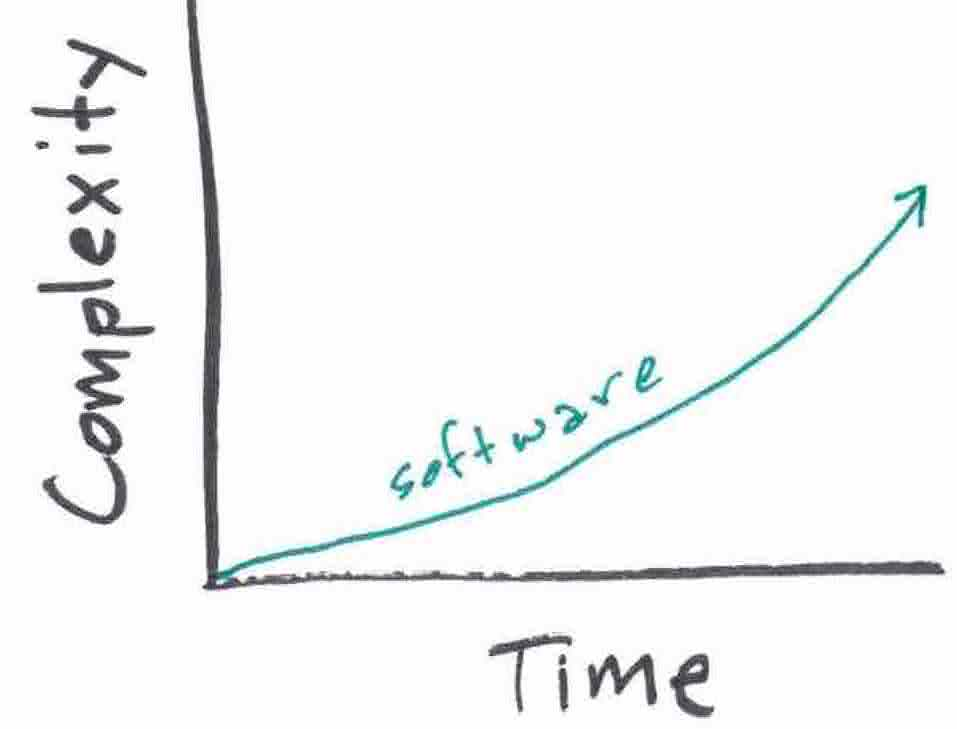
\includegraphics[width=0.7\columnwidth]{TimeAndComplexity}
    }
    \caption{Generally speaking, a software system will get more complex as it grows over time.}
    \label{figTimeAndComplexity}
\end{figure}

One way to understand the quality around a system is to discuss its ``maintainability,'' the ease of receiving new features or resolving bugs. For example, if a system is tightly coupled, it may be that adjusting one area to add a new feature requires touching several other parts of the system.

To give some simple examples for tightly and loosely coupled systems, let us consider a person's eyes. If the person is a near-sighted individual, a loosely coupled solution to improve that person's vision is to get glasses or contacts. They can change the glasses for different types and styles while solving the problem (poor vision). However, they cannot simply change their eyes; the eyes are tightly coupled to a person's body and would be difficult to remove and swap for another set of eyes without considerable work to separate and reattach them to the correct systems. By having a loosely coupled system (wearing glasses), we allow for easy feature changes (turn those glasses into sunglasses! pick a new style!) and easy bug fixes (adjust the prescription).

Like how it may be easier to change how we look and how well we can see by using prescriptive eyewear, creating a structured software system will impact how the software can evolve with new features. If a system is difficult to evolve, users will lose favor with that system as it cannot offer features that are comparable to their competitors (\ref{sectionTheProblem}).

% --- SUMMARY OF CONTRIBUTIONS ------------------------------------------------
% --- How does my idea solve the problem? -------------------------------------
% --- THE PROBLEM: Some projects fail to evolve, resulting in loss if income.
% --- MY IDEA: Software evolution is impacted by structural quality.
% -----------------------------------------------------------------------------

We will explore automated measurements that provide evaluation scores of software systems. By using some of these quality and maintainability scores, we can see how structure impacts evolution (Section \ref{sectionMyIdea}). In our case, we will explore the Pylint Refactor score on commits for new features, focusing specifically on the adaptability and evolution of a software project (Sections \ref{sectionSoftwareData} and \ref{sectionMaintainabilityScores}).

When a team is able to embrace and use these types of measurements from the beginning of a project, it enables faster architecture review than checking it only by hand. These types of measurements can inform us of areas with ``smells,'' providing insight on where to focus on improvements. In addition to the usefulness at the beginning of a project, continuing to revisit these numbers on a regular basis (every sprint, for example, in a scrum team) keeps the project in a maintainable state.

% \todo{TODO: what is the specific, refutable information that we found?}

In addition to using scores to predict software evolution ability, we also look at documentation used in the best and worst projects to determine that good documentation can improve maintainability (Section \ref{sectionDocumentation}).

% =============================================================================
% =  The Problem (1 page)
% =============================================================================

\vspace{0.5cm}
\section{Keeping Users Engaged Long Term} \label{sectionTheProblem}
\vspace{0.25cm}

% --- The problem is that some projects fail to evolve ------------------------

When developing a new system or a new software idea, getting the project off the ground and in front of users is one thing. However, keeping that project alive with a thriving community of engaged users is another.

The systems we create could be customer-facing web applications, games, or internal applications used to carry out tasks. Regardless of the type of system, the product will no longer provide usefulness without evolving with the user's needs. Even in a corporate setting with internal business systems, over time, users will need change; how a system can adapt to those needs requires a level of flexibility.

\vspace{0.25cm}
\begin{displayquote}
``Software evolution is the continual development of software after its initial release to address changing stakeholder and/or market requirements.'' \cite{wiki:software-evolution}
\end{displayquote}
\vspace{0.25cm}

% --- Why does it matter if a project does not evolve? ------------------------
\vspace{0.25cm}
\subsection{Why does software evolution matter?}

When a system cannot evolve, the impact is primarily felt by the users. However, this impact will eventually get back to those who created and continue to support the system. With users that are either unsatisfied or unable to use the system any longer, the engagement levels will drop. The decline in users will ultimately result in a loss of income, as the system can no longer deliver to the needs of its audience.

Because organizations invest large amounts of money in the software systems that they create, they depend on the software's continued success. Software evolution will allow the system to adapt to new or changing business requirements, fix bugs and defects, and integrate with other systems that have changed and evolved that may share the same software environment.

As a system is used, inevitably, users will stumble into situations that even the best quality assurance testers will miss. When defects are found, they will require fixing. 

To keep a system up-to-date, we must add new features. For example, there may be a need to improve a system's performance or reliability, especially if the user base expands.

Security can also impact the need for a system to be maintained. New ways to infiltrate a system can be uncovered, so it is important to stay on top of newest versions of dependencies and technologies in order to avoid potential breaches of data and experience.

% --- How do we ensure a project will be able to evolve? ----------------------
\vspace{0.25cm}
\subsection{How do we ensure software evolution?}

Because the maintainability of a system can ultimately influence the ability to generate revenue, we must find ways to ensure that a project will evolve. One of these ways could be to ensure that a project continues to be considered ``maintainable'' throughout its lifetime. This system characteristic will ensure that bugs can be fixed quickly, but new features should be easy to add as the users' needs evolve.

If a system is extensive, it may involve many steps to get changes through. For example, a process like that in ``Fig.~\ref{figSystemMaintenance}'' shows steps to get to a new minor feature release. Any amount of complexity can make this multi-step process even more cumbersome.

\begin{figure}[ht]
    \centerline{
        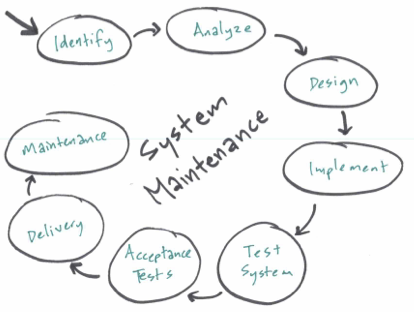
\includegraphics[width=0.8\columnwidth]{Maintenance}
    }
    \caption{The general steps followed when implementing bug fixes or minor enhancements in a system.}
    \label{figSystemMaintenance}
\end{figure}

If we look at the process for System Evolution, we see that it is very similar to what we find with standard maintenance steps (``Fig.~\ref{figSystemEvolution}'').

\begin{figure}[ht]
    \centerline{
        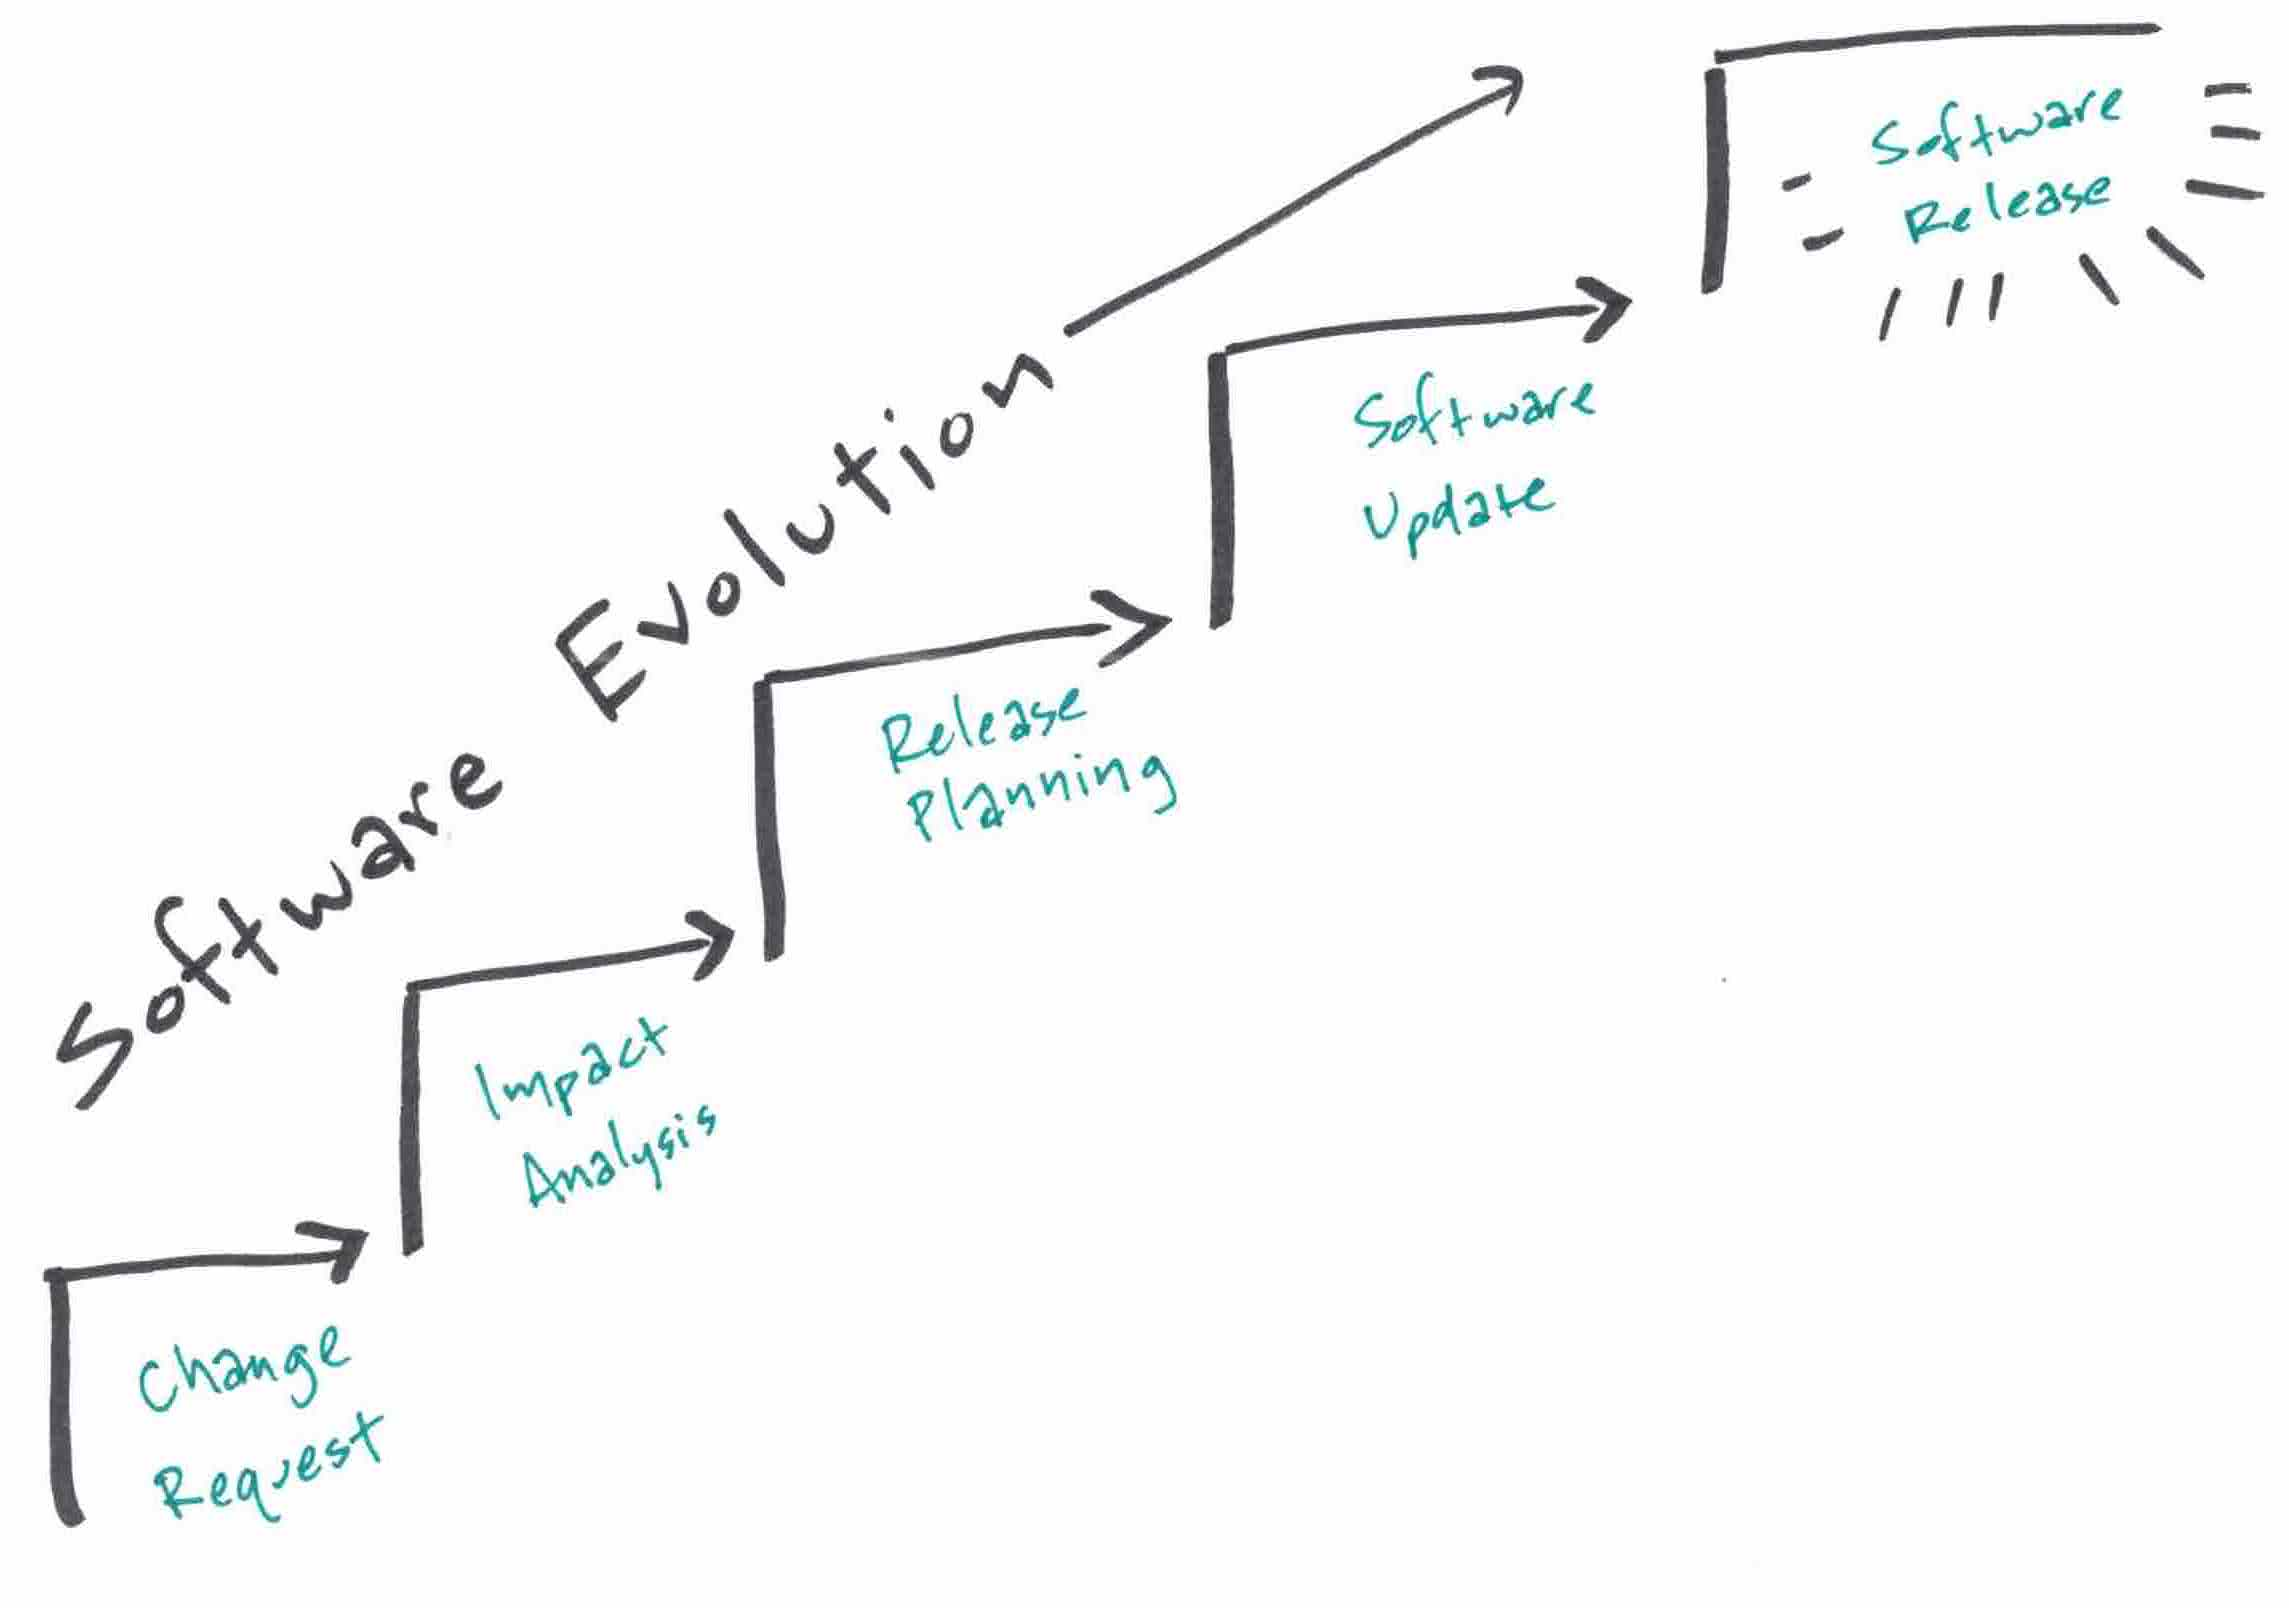
\includegraphics[width=0.8\columnwidth]{Evolution}
    }
    \caption{The general steps followed when adapting or migrating a system.}
    \label{figSystemEvolution}
\end{figure}

% =============================================================================
% =  My Idea (2 pages)
% =============================================================================

\vspace{0.5cm}
\section{The Impact of Structural Quality} \label{sectionMyIdea}
\vspace{0.25cm}

% --- Understand Software Maintenance -----------------------------------------
\vspace{0.25cm}
\subsection{Software Maintenance}

The structural quality of a software system will impact the software evolution. If the project has poor structural quality, its ability to evolve will be minimized, and the software system will eventually ``die-off'' so to speak.

There is much planning involved in all software creation projects in what the product will be, will do, who it is for, etc. One of the things that should also be on the planning list is long-term maintenance and growth. That is, how do we build a thing that will be easier to add features to down the road?

Let us define maintainability in the context of software. For example, a system would be considered easy to maintain if it is easy to debug and easy to add new features. These new features are generally considered minor features, and may often be reported as bugs by users, when in reality, they are looking for functionality enhancements \cite{wiki:software-maintenance}.

\vspace{0.25cm}
\begin{displayquote}
``Software maintenance in software engineering is the modification of a software product after delivery to correct faults, to improve performance or other attributes.'' \cite{wiki:software-maintenance}
\end{displayquote}
\vspace{0.25cm}

It may be easier to understand what characteristics define a system with poor maintainability. These types of systems will have poor code quality, leading to defects. For example, there could be undetected vulnerabilities or vulnerabilities that have been ignored. It may be that the system is overly complex. In addition to the complexity, it could be hard to read due to poor naming or dead (unused) code throughout the source code.

A project is known to have good maintainability when there is an enforced set of clean and consistent standards for the code. This often involves having human-readable names for functions, methods, and variables. Any complex code is minimized, and methods are small and focus on a single thing. Parts of the system are decoupled and organized, making it easy to work on different parts with low impact on unrelated parts. For example, the code is DRY (there is limited redundancy in the code), unused code has been removed, and there is a level of documentation that supports an easy understanding of the system.

Why should we care about whether the code is maintainable? It is assumed that a large amount of the cost over the lifetime of a project is attributed to maintainability. Fred Brooks, in his book ``The Mythical Man-Month'' even claimed that over 90\% of the costs for a typical software system come up in the maintenance phase \cite{brooks:mythical}. Once the bulk of the system is off the ground and live worldwide, how well the team can improve the system with new features and fix bugs, even working on different parts in parallel, can be impacted by its maintainability. Any successful piece of software will inevitably need to be maintained.

% --- Understand Software Evolution -------------------------------------------
\vspace{0.25cm}
\subsection{Software Evolution}

There is a distinction to be made between \textbf{software maintenance} and \textbf{software evolution}. We will refer to software maintenance as bug resolution and for minor functional improvements. For example, we can consider this routine maintenance when we must fix a broken route in the application or provide a subtle enhancement on the user experience. However, when we look at upgrades to the system, adaptations to the changing and growing needs of the user, or migrating the system to a new technology, we can refer to this as evolution of the software.

The evolution of software can result from new laws that have come into being. As technology itself changes, governing bodies must continually revisit data collection and information sharing policies. Changes in technology and laws may lead to adaptations in the software systems.

It is also fair to say that systems will change because we can never fully determine a user's needs at the start of a project. It would be safe to say that the user's needs will change over time themselves. This leads to a never-ending project that will always need some form of enhancement.

Meir ``Manny'' Lehman and László ``Les'' Bélády contributed to a list of laws involving software evolution known as Lehman's Laws that describe a balance between forces that drive new developments while also slowing progress. These laws apply to programs that were written to perform some real-world activity, where its behavior is linked to the environment in which it runs; additionally, this program category assumes that the program needs to adapt to varying requirements and circumstances in that environment. Eight laws were created and are listed below. \cite{wiki:lehmans-laws}

\vspace{0.25cm}
\begin{enumerate}
    % "Continuing Change" — an E-type system must be continually adapted or it becomes progressively less satisfactory.
    \item \textbf{Continuing Change} \textit{(1974)}
    
    % "Increasing Complexity" — as an E-type system evolves, its complexity increases unless work is done to maintain or reduce it.
    \item \textbf{Increasing Complexity} \textit{(1974)}

    % "Self Regulation" — E-type system evolution processes are self-regulating with the distribution of product and process measures close to normal.
    \item \textbf{Self Regulation} \textit{(1974)}

    % "Conservation of Organisational Stability (invariant work rate)" — the average effective global activity rate in an evolving E-type system is invariant over the product's lifetime.
    \item \textbf{Conservation of Organisational Stability} \textit{(1978)}

    % "Conservation of Familiarity" — as an E-type system evolves, all associated with it, developers, sales personnel, and users, for example, must maintain mastery of its content and behavior to achieve satisfactory evolution. Excessive growth diminishes that mastery. Hence the average incremental growth remains invariant as the system evolves.
    \item \textbf{Conservation of Familiarity} \textit{(1978)}

    % "Continuing Growth" — the functional content of an E-type system must be continually increased to maintain user satisfaction over its lifetime.
    \item \textbf{Continuing Growth} \textit{(1991)}

    % "Declining Quality" — the quality of an E-type system will appear to be declining unless it is rigorously maintained and adapted to operational environment changes.
    \item \textbf{Declining Quality} \textit{(1996)}

    % "Feedback System" (first stated 1974, formalised as law 1996) — E-type evolution processes constitute multi-level, multi-loop, multi-agent feedback systems and must be treated as such to achieve significant improvement over any reasonable base.
    \item \textbf{Feedback System} \textit{(1996)}
\end{enumerate}
\vspace{0.25cm}

The first law, ``Continuing Change,'' tells us that if a system does not adapt, it will become progressively less satisfactory. The second, ``Increasing Complexity,'' explains that as a system evolves, unless work is done to maintain or reduce complexity, the complexity will increase (``Fig.~\ref{figTimeAndComplexity}'' again). This can be due to the added volume of the code from new features or even an increasing number of developers that have edited the code. Unless this phenomenon of increased complexity is actively addressed during changes, it can impact the maintainability (and the ability of a project to continue evolving) in the future.

Lehman's fifth law, ``Conservation of Familiarity,'' explains how the average incremental growth does not change over time as a system evolves. The people interacting with the system, such as the developers, business persons, or users, must still continue using and working within the system at the same ``level of mastery.'' If the system grows and changes excessively, the mastery will drop, slowing down the next set of changes. This could be because the source code or architecture has become more complex (impacting the developers' ability to adapt and enhance the system) or because the user features have changed so that the system audience needs time to master the new interfaces or new tools. Because of this natural ``slow-down'' for excessive change, the average incremental growth will remain steady. We can see a simplified visual in ``Fig.~\ref{figConservationOfFamiliarity}'' showing that when the number of changes spikes (that is to say, when there is excessive growth in a system), it will be followed by an iteration of fewer changes, leading to a nearly consistent average of incremental growth (the thick, horizontal line) over time.

\begin{figure}[ht]
    \centerline{
        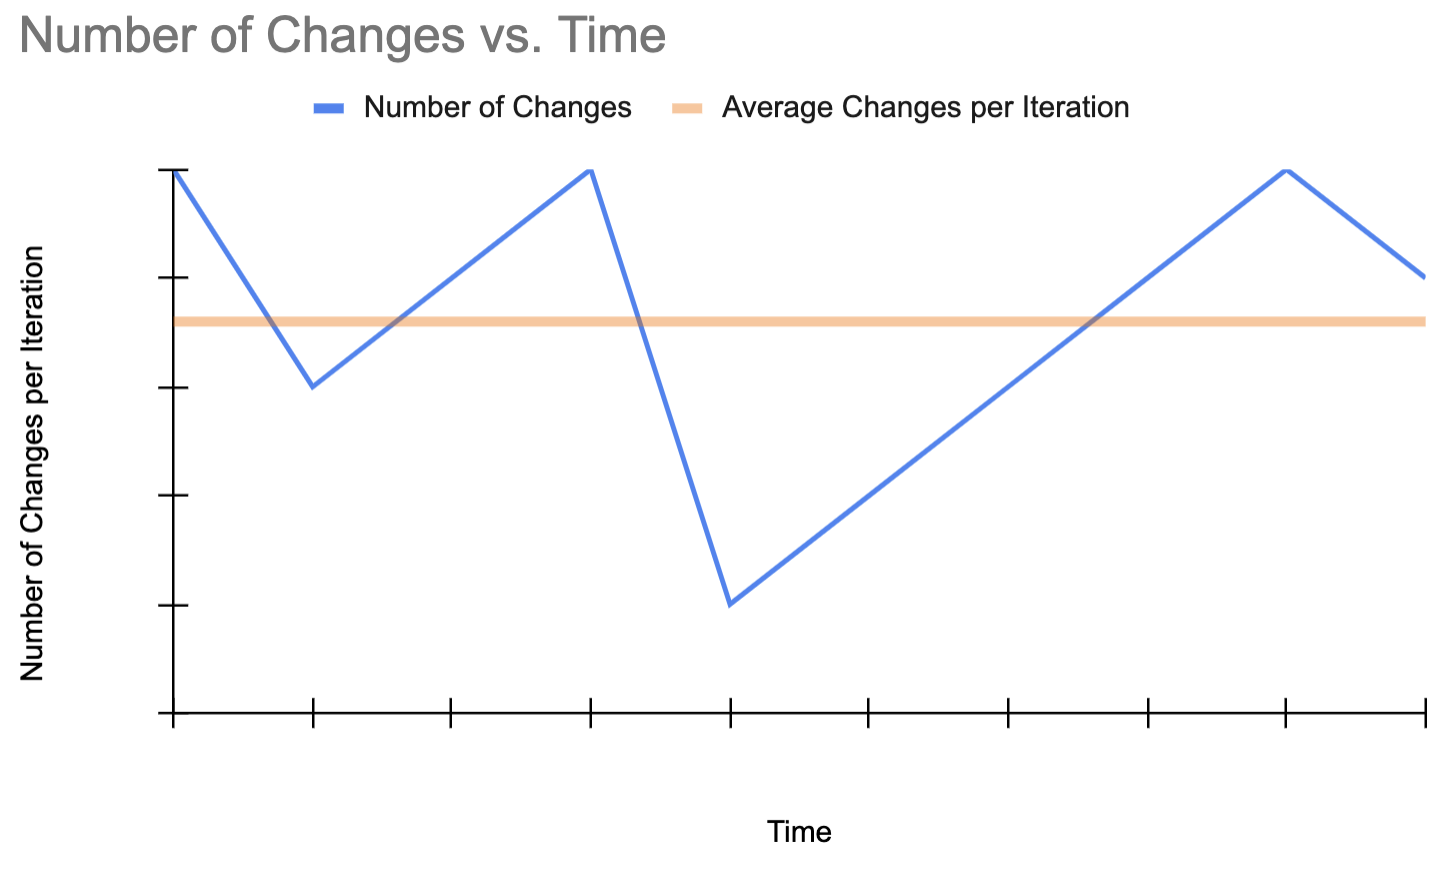
\includegraphics[width=\columnwidth]{Changes-vs-Time}
    }
    \caption{A simplified visual of Lehman's fifth law, ``Conservation of Familiarity.''}
    \label{figConservationOfFamiliarity}
\end{figure}

In Lehman's sixth law, ``Continuing Growth,'' we see that the system user's satisfaction will not be maintained without continually increasing the functional content. Along a similar idea, the law pertaining to ``Declining Quality'' states that if the operational environment for the system does not change, the system's quality will appear to decline. Therefore, we must continue adapting for even the appearance of the maintained quality of a system.

With all of these characteristics surrounding the evolution of software, we benefit from the Internet that has positively improved the experience. Two common resources currently available to developers have impacted software evolution \cite{wiki:software-evolution}:

\vspace{0.25cm}
\begin{enumerate}
    \item The rapid growth of the World Wide Web and Internet Resources make it easier for users and engineers to find related information.
    \item Open source development where anybody could download the source codes and modify it has enabled fast and parallel evolution (through forks).
\end{enumerate}
\vspace{0.25cm}

These two suggestions are very evident in modern development. For example, a developer may regularly use resources like StackOverflow to find solutions to problems and use open-source tools that the developer and their team can contribute to or adjust to their specific needs.

\vspace{0.25cm}
\subsection{Measuring Maintainability}

Despite the nuanced differences between \textit{maintainability} and \textit{evolution}, the two characteristics run parallel to each other. If a system is easy to maintain, it will also be easier to evolve. If we can measure our system's maintainability, we can also determine if our system is in a good position to continue evolving to meet our future needs.

Several tools attempt to provide some value around these ideas. In this paper, we will focus on the metrics that Pylint provides, specifically looking into the Refactor score of Pylint.

We will look at many open-source Python systems using Pylint and attempt to correlate the data from the Pylint scores to the level of ease in adding new features to the system. This will determine if a system is more maintainable with better Pylint scores. 
% \todo{FUTURE EDITION: To do this, we will measure the locality of the changes by the number of files that are edited in a commit. We will also focus on commits that represent new features, not on commits that are bug fixes.}

% =============================================================================
% =  The Details, defending my idea (5 pages)
% =============================================================================

\vspace{0.5cm}
\section{Reviewing Python Software Projects}
\vspace{0.25cm}

% --- How does my idea solve the problem? -------------------------------------
% --- THE PROBLEM: Some projects fail to evolve, resulting in loss if income.
% --- MY IDEA: Software evolution is impacted by structural quality.
% -----------------------------------------------------------------------------

We have established that we have a problem with projects that fail to evolve, resulting in a loss of revenue. We also understand that evolving software is essential in order to keep users engaged; without it, there is an appearance in the decline of quality and the program becomes less satisfactory to the user, as well as potential for competitors to outpace us with features available. We must now understand how we can ensure that our systems evolve. For this, we will look to understand how the system's structural quality impacts software evolution.

% -----------------------------------------------------------------------------
% -  (A) We can use maintainability scores to see how structure impacts evolution.
% -----------------------------------------------------------------------------
\vspace{0.25cm}
\subsection{Open Source Software Systems} \label{sectionSoftwareData}

% --- Claim A: Review each claim from the introduction
On order to gain better understanding of software systems and the metrics we seek to use in order to understand the quality of the software structure, we scanned a collection of open source Python systems from GitHub. There were 129 repositories that were downloaded and the Pylint report was applied to each.

Of these repositories, we found there were a total of 88 different messages called out. There were 52 messages categorized as \emph{refactor} warnings and 35 flagged for \emph{conventions} that should be used.

When measuring the Refactor score, we are looking at the number of lines of code called out with Refactor warnings. Smaller scores are better (fewer warnings). The ``best'' repository in regards to Refactor scores was \emph{Munki} with the lowest Refactor at 8 \cite{data:munki}. This repository has only 82 contributors.

The repository for \emph{Ansible}, on the other hand, scored the worst in the batch, with a Refactor score at 16990 \cite{data:ansible}. However, this repository has over 5,000 contributors, which emphasizes the difficulty in keeping a project on track in regards to low technical debt.

% --- Claim A: Identify the evidence (analysis and comparison, theorems, measurements, case studies)

% \todo{TODO: examples or evidence?}

% -----------------------------------------------------------------------------
% -  (B) We can use maintainability scores to see how structure impacts evolution.
% -----------------------------------------------------------------------------
\vspace{0.25cm}
\subsection{Maintainability Scores} \label{sectionMaintainabilityScores}

% --- Claim B: Review each claim from the introduction

First, let us consider our original understanding of software maintainability. While this definition focuses primarily on bug fixes and minor enhancements, maintainable projects should also have ease in their ability to evolve. Therefore, we can study the impact maintainability (structural quality) has on software evolution by reviewing the scores provided by automated code review tools.

In this study, we will be using Pylint and will be focused on the values of the Refactor score regarding a set of open-source Python systems. To understand the scores we will be working with, we must understand what Pylint itself is doing. 

Through the documentation of Pylint, we can understand how to use it and the scores it will provide \cite{pylint:main}. The Pylint score itself is calculated by the following equation \cite{pylint:score}:

\vspace{0.25cm}
\code{10.0-((float(5*e+w+r+c)/s)*10)}
\vspace{0.25cm}

Numbers closer to \code{10} reflect systems that have fewer errors, fewer warnings, and have overall better structure and consistency. In the above equation, we are using the following values \cite{pylint:docs}:

\vspace{0.25cm}
\begin{itemize}
    \item \textbf{statement} (\code{s}): the total number of statements analyzed
    \item \textbf{error} (\code{e}): the total number of errors, which are likely bugs in the code
    \item \textbf{warning} (\code{w}): the total number of warnings, which are python specific problems
    \item \textbf{refactor} (\code{r}): the total number of refactor warnings for bad code smells
    \item \textbf{convention} (\code{c}): the total number of convention warnings for programming standard violations
\end{itemize}
\vspace{0.25cm}

The Refactor score is of special interest to us and considers many features that are meticulously outlined on the Pylint site \cite{pylint:refactor}. These types of warnings include a number of checks, such as when a boolean condition could be simplified, or a useless \code{return}, and so on. This score, in particular, will be part of our focus.

To calculate the Refactor score, Pylint will check the code for code smells based on the definitions for checks that have been documented. For every infraction, the score increases by one count. 

% -- How Pylint Refactor errors are related to architecture smells ------------

\vspace{0.25cm}
\begin{displayquote}
``In computer programming, a \textbf{code smell} is any characteristic in the source code of a program that possibly indicates a deeper problem.'' \cite{wiki:code-smells}
\end{displayquote}
\vspace{0.25cm}

% \todo{TODO: expand on this idea more}
We can use these Refactor scores to help us spot architecture smells. After all, code smells can point the way to deeper problems in our system. There are fundamental design principles that have been established that we should consider when creating software; code smells alert us to areas that have deviated from these principles. These smells are drivers for refactoring and, when addressed, can help us maintain the integrity of our architecture rather than creating a patchwork construction.

% -- Examples from our data set of the most common Refactor messages ----------
Because of the relation of refactor scores to the code structure itself, we will be spending much of our focus on this particular value. The most common Refactor error returned in our data set was the \code{no-else-return} message. This particular message highlights when an unnecessary block of code follows an if-statement that contains a \code{return}. The second most common Refactor message was \code{too-few-public-methods}, which reminds the developer to consider whether that class is appropriate to create.

Finally, in respect to Python, it is also helpful to be familiar with PEP 8, as this is the default set of standards that Pylint uses to judge Python code \cite{pylint:pep8}. This standard can be used to make code more readable and more consistent, which may contribute to the code being more maintainable. These standards cover things like indentation spacing, maximum line length, where to break lines, how to handle imports, and more. By defining a set of standards, teams can ensure they have a defined set of rules so that any contributors to the code understand the expectations (and so that automated systems like Pylint can enforce those standards to maintain readability and consistency).

% --- Claim B: Identify the evidence (analysis and comparison, theorems, measurements, case studies)

\vspace{0.25cm}
\subsection{Other Maintainability Characteristics}

The authors of ``Measurement and refactoring for package structure based on complex network'' recently reviewed a similar idea focusing on cohesion and coupling over time for a project \cite{zhou:2020}. In a software system, we desire low coupling (allowing for changes to one area to remain independent of changes to another area) and high cohesion (indicating reduced complexity in modules, which improves maintainability). Through a few experiments on open-source software systems, the authors determined that their algorithm that calculated metrics was capable of improving package structures to have high cohesion and low coupling. Their study gives us confidence that metrics around the software's structure can provide value in keeping systems in a maintainable state, which allows for software evolution.

Another variable that may impact the maintainability of code is readability. For example, in the article ``How does code readability change during software evolution?'' the authors have addressed this concern and found that most source codes were readable within the sample they reviewed. Additionally, a minority of commits changed the readability; if a file was created as less readable, it was likely that it remained that way and did not improve \cite{piantadosi:2020}. This variable (readability) in the maintainability of a software system can influence how easy or difficult it is to make a change. The authors also found that big commits, usually associated to adaptive changes (a form of software evolution), were the most prone to reduce code readability \cite{piantadosi:2020}. This assumes that smaller commits are almost always better and can lead to more readable code.

Piantadosi et al. found that changes in readability, whether improvements or disintegrations, often occurred unintentionally \cite{piantadosi:2020}. By enforcing the PEP 8 standard, we know that Pylint is encouraging systems to remain readable. Therefore, projects that use some form of automated system in their pipeline benefit from keeping their project on track in this regard, limiting the effects of readability on a software's potential for evolution.

The paper ``Standardized code quality benchmarking for improving software maintainability'' provides additional insights into how the code's maintainability is impacted by the technical quality of source code \cite{baggen:2012}. Within their paper, the authors seek to show four key points: (1) how easy it is to determine where and how the change is made, (2) how easy it is to implement the change, (3) how easy it is to avoid unexpected effects, and (4) how easy it is to validate the changes. Their approach has shown that some tools and methods can be used to improve and maintain technical quality within their projects, allowing systems to continue to evolve at a reasonable pace.

% -----------------------------------------------------------------------------
% -  (C) Documentation can improve maintainability.
% -----------------------------------------------------------------------------
\vspace{0.25cm}
\subsection{Documentation} \label{sectionDocumentation}

% --- Claim C: Review each claim from the introduction

Our assumption is that the Refactor score in projects should correlate to the evolution of the system. The first pass through the data is not conclusive in this particular detail, as the projects reviewed have many other factors contributing to the evolution of the project (number of contributors, size of the code system, etc.). Our assumption is that the correlation between software quality and software evolution would indicate that the better-scoring code systems are readable in themselves. In addition, it would be helpful to understand whether there are any similarities in how a system is documented that could contribute to improved software evolution of a system.

% \todo{TODO: what kind of documentation do the ``good'' projects have?}

% \todo{TODO: what kind of documentation do the ``bad'' projects have?}

% --- Claim C: Identify the evidence (analysis and comparison, theorems, measurements, case studies)

The course textbook, ``Software Architecture in Practice,'' chapter 18 provides some insight in documentation around architecture \cite{book:software-architecture-in-practice}:

\vspace{0.25cm}

\begin{displayquote}
``If you go to the trouble of creating a strong architecture, one that you expect to stand the test of time, then you \textit{must} go to the trouble of describing it in enough detail, without ambiguity, and organizing it so that others can quickly find and update the needed information.''
\end{displayquote}

\vspace{0.25cm}

The book describes how documentation holds the results of significant design decisions, providing valuable insights into decisions down the road. While not directly related to the Pylint Refactor score and not within the source code itself, it is still helpful to remind ourselves that documentation can also influence the ability of a software system to evolve.

Our ``best scores'' (regarding the current Pylint Refactor score) were found to have relatively organized and useful documentation. The code repository for \emph{Munki} provided documentation for previous versions, lending insight into design decisions as the software evolved \cite{data:munki}. The repository for \emph{Raven}, however, was a deprecated version that has since been replaced by a paid platform known as \emph{Sentry}, but had ample documentation \cite{data:raven-python}. It is possible that the ``death'' of that software system was not lack of evolution, but rather a business decision. \emph{ElastAlert} was another system with good scores and easy-to-follow documentation, though it is focused more for the use of the system rather than how to enhance the system itself \cite{data:elastalert}.

When reviewing our ``worst offenders'' in current Refactor scores, it was noted that even with poor scores, these repositories were able to continue to see engagement from developers. While further inspection will be needed to understand whether the code itself is evolving or just has engagement from a maintenance level, it is interesting to note that there is decent documentation provided. \emph{SymPy} goes as far as documenting the architecture for the software as well as design decisions, enabling developers to better understand the structure as they make contributions \cite{data:sympy-docs}.

\vspace{0.25cm}

\begin{displayquote}
``Our study has shown that the primary studies provide empirical evidence on the positive effect of documentation of designs pattern instances on programme comprehension, and therefore, maintainability.''
\end{displayquote}

\begin{displayquote}
``...developers should pay more effort to add such documentation, even if in the form of simple comments in the source code.''
\end{displayquote}

\vspace{0.25cm}

In research done by Wedyan and Abufakher (quoted above), it was found that documenting design patterns was useful in enhancing code understanding \cite{wedyan:2020}. In turn, the comprehensibility impacts the maintainability of the code in a positive way, which continues to reinforce the impact that documentation can have and how it ties well into considerations for software structure.

% =============================================================================
% =  Related Works (1 to 2 pages)
% =============================================================================

\vspace{0.5cm}
\section{Related Work}
\vspace{0.25cm}

The work done by Dr. Omari and Dr. Martinez involves collecting a sub-set of Python projects that we can use for further research. The bulk of the effort they have provided is determining which classifiers to use to pare down the public set of Python systems into a good collection for further analysis \cite{omari:2018}. The work that they have provided was used to select appropriate Python systems for review by collecting meta-data on these code systems.

From their subset of repositories, we were then able to collect current Pylint scores from each of our 129 systems. This gives us a sampling of data that we can now dig deeper into, comparing similar systems (similar size, similar number of contributors, etc.) and their evolution process by reviewing past commits rather than merely the current state of the system, as we have done here.

In the paper ``Impact of design patterns on software quality: a systematic literature review'' the authors compared the use of design patterns to software evolution and maintainability. They found that design patterns provided clear flexibility when they reviewed changes that extended (evolved) software \cite{wedyan:2020}.

\vspace{0.25cm}

\begin{displayquote}
``Changes performed in a class can be corrective, adaptive, perfective, or preventive. These changes can occur due to new requirements, debugging, changes that propagate from changes in other classes and refactoring.''
\end{displayquote}

\vspace{0.25cm}

Wedyan and Abufakher found that there were two reasons that a class had more frequent changes \cite{wedyan:2020}:

\vspace{0.25cm}

\begin{enumerate}
    \item The class was easy to extend.
    \item The class correlated to other classes (raising alarms about class modularity).
\end{enumerate}

\vspace{0.25cm}

With these findings in mind, we intentionally aim to focus future research on changes for system extensions and adaptations rather than bug fixes that appeared to be larger change due to high coupling. Within this paper, we were able to focus on Refactor scores (code smells) rather than Error scores (bugs) within the system.

% =============================================================================
% =  Conclusions and Further Work (0.5 page)
% =============================================================================

\vspace{0.5cm}
\section{Conclusions \& Further Work}
\vspace{0.25cm}

By collecting data and drawing our conclusions from it, with help from the insights from the studies done before ours, we may better understand metrics that can be useful regarding maintainability. Good projects will inevitably continue to grow and evolve. Understanding methods to keep code refactor on a certain level makes code easy to change. We may also find that projects with worsening scores slow down with updates and have reduced engagement.

When reviewing our surface-level data with current project Refactor scores, our three worst offendors were \emph{Ansible} \cite{data:ansible}, \emph{SymPy} \cite{data:sympy}, and \emph{Salt} \cite{data:salt}. All three projects are still quite active with development despite their poor current scores. The projects have high download rates, which may be the reason for continued development despite potential difficulty in maintenance. 

Projects that may be open source or have many contributors are especially vulnerable to maintainability degrading over the evolution of a project. Having a reliable metric can be very useful in programmatically avoiding code smells and keeping code in a state that is easy to manage through simple metric checks in deployment pipelines.

We can see an example of this in reviewing some current symptoms that \emph{SymPy} is experiencing, with only 72\% code coverage and a failing build (see ``Fig.~\ref{figSymPyStatus}''). Despite the engagement and continued development, we suspect that real adaptations and evolution of the software may be difficult with this code.

\begin{figure}[ht]
    \centerline{
        
\includegraphics[width=1.0\columnwidth]{SymPy_status}
    }
    \caption{A snapshot of the badges from \emph{SymPy}'s repository.}
    \label{figSymPyStatus}
\end{figure}

We have further work to do in this study to gain better understanding. With a set of several ``best'' and ``worst'' Python software systems, we will look into the history of the projects' commits. It would be useful to see how the Refactor scores have changed over time, and if the rate at which changes were pushed correlated to the increase or decrease in that Refactor score. 

Additional data can be gathered from this set that may provide more insights than this first brush of the data provides us. Understanding the impact of structural quality on the evolution of a project can provide compelling perspectives.

% =============================================================================
% =  Bibliography and Sources
% =============================================================================
\newpage

% Set line spacing for Bibliography
\setstretch{1.4}

\bibliographystyle{unsrt}
\bibliography{bibliography}

% =============================================================================
% =  END OF THE DOCUMENT
% =============================================================================
\end{document}
